\documentclass[journal,13pt,twocolumn]{IEEEtran}

\usepackage{setspace}
\usepackage{gensymb}
\counterwithin{equation}{section}
\singlespacing

\newcommand{\myvec}[1]{\ensuremath{\begin{pmatrix}#1\end{pmatrix}}}
\usepackage[cmex10]{amsmath}
\usepackage{amsthm}
\usepackage{mathrsfs}
\usepackage{txfonts}
\usepackage{stfloats}
\usepackage{bm}
\usepackage{cite}
\usepackage{cases}
\usepackage{subfig}
\usepackage{longtable}
\usepackage{multirow}
\usepackage{mathtools}
\usepackage{steinmetz}
\usepackage{tikz}
\usepackage{circuitikz}
\usepackage{verbatim}
\usepackage{tfrupee}
\usepackage[breaklinks=true]{hyperref}
\usepackage{tkz-euclide} % loads  TikZ and tkz-base
%\usetkzobj{all}
\usetikzlibrary{calc,math}
\usepackage{listings}
    \usepackage{color}                                            %%
    \usepackage{array}                                            %%
    \usepackage{longtable}                                        %%
    \usepackage{calc}                                             %%
    \usepackage{multirow}                                         %%
    \usepackage{hhline}                                           %%
    \usepackage{ifthen}                                           %%
  %optionally (for landscape tables embedded in another document): %%
    \usepackage{lscape}     
\usepackage{multicol}
\usepackage{chngcntr}
\usepackage{pgfplots}
\usepackage{pgfplotstable}
\pgfplotsset{compat=1.7}
\usepackage{tikz}
\DeclareMathOperator*{\Res}{Res}
\renewcommand\thesection{\arabic{section}}
\renewcommand\thesubsection{\thesection.\arabic{subsection}}
\renewcommand\thesubsubsection{\thesubsection.\arabic{subsubsection}}

\renewcommand\thesectiondis{\arabic{section}}
\renewcommand\thesubsectiondis{\thesectiondis.\arabic{subsection}}
\renewcommand\thesubsubsectiondis{\thesubsectiondis.\arabic{subsubsection}}

\DeclarePairedDelimiter\abs{\lvert}{\rvert} % \abs{} for numerisk værdi
\DeclarePairedDelimiter\norm{\lVert}{\rVert}
\makeatletter
\let\oldabs\abs
\def\abs{\@ifstar{\oldabs}{\oldabs*}}
\let\oldnorm\norm
\def\norm{\@ifstar{\oldnorm}{\oldnorm*}}
\makeatother
\renewcommand{\vec}[1]{\mathbf{#1}}
\newcommand{\bignorm}[1]{\Bigl \| #1 \Bigr \| #1}
\hyphenation{op-tical net-works semi-conduc-tor}
\def\inputGnumericTable{}                                 %%

\lstset{
frame=single, 
breaklines=true,
columns=fullflexible
}
\begin{document}
\title{Assignment 2} 
\author{Shweta Verma} 
\maketitle
\newpage
\bigskip
\begin{abstract}
This document solves a problem based on the inclination of straight lines
\end{abstract}
\section{\textbf{Problem}}
If the lines
\begin{align}
\myvec{-3 & 1} \vec{x} = 1\\ 
\myvec{-1 & 2} \vec{x} = 3
\end{align}
are equally inclined to the line 
\begin{align}
\myvec{-m & 1} \vec{x} = 4
\end{align}
Find the value of m.
\section{\textbf{Solution}}
  To find the angle between two lines we use-
 \begin{align}
 \cos\theta = \frac{a^T b}{||a||~||b||}
 \end{align}
 Assume line(1.1), (1.2) and (1.3) as vectors $\vec{a}$,$\vec{b}$ and $\vec{c}$ respectively
 \begin{align}
 \vec{a} = \myvec{-3 \\ 1}\\
 \vec{b} = \myvec{-1 \\ 2}\\
 \vec{c} = \myvec{-m \\ 1}
 \end{align}
 \begin{align}
  |\vec{a}| = \sqrt{10}
 \end{align} 
 \begin{align}
  |\vec{b}| = \sqrt{5}
 \end{align} 
 \begin{align}
  |\vec{c}| = \sqrt{m^2+1}
 \end{align} 
  \begin{align}
  \vec{a}^T \vec{c} = 3m+1
  \end{align}
  \begin{align} 
  \vec{b}^T \vec{c} = m+2
 \end{align} 
 Angle between $\vec{a}$ and $\vec{c}$ using (2.1)
 \begin{align}
  \cos\theta = \frac{3m+1}{\sqrt{10}\sqrt{m^2+1}}
 \end{align}
  Angle between $\vec{b}$ and  $\vec{c}$ using (2.1)
 \begin{align}
 \cos\theta = \frac{m+2}{\sqrt{5}\sqrt{m^2+1}}
 \end{align}
  According to question
  $\vec{a}$ and $\vec{b}$ are equally inclined to $\vec{c}$
  Therefore, (2.10) and (2.11) are equal
  \begin{align}
  \frac{3m+1}{\sqrt{10}\sqrt{m^2+1}} = \frac{m+2}{\sqrt{5}\sqrt{m^2+1}}
  \end{align}
  \begin{align}
  \implies \frac{3m+1}{\sqrt{2}} = m+2
  \end{align}
   \begin{align}
   \implies m = \frac{1+5\sqrt{2}}{7}
   \end{align}    
   \begin{figure}
   \centering
   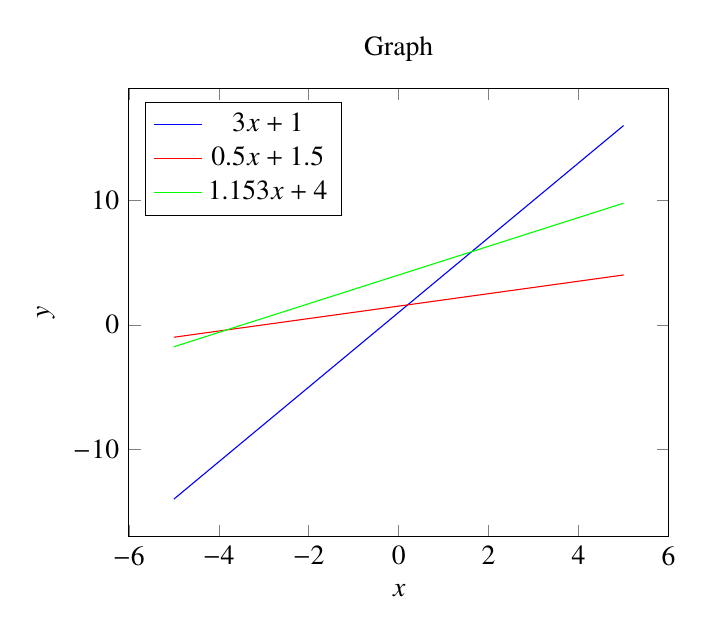
\begin{tikzpicture}
   \begin{axis}[
   legend pos=north west,
   title=Graph,
   xlabel={$x$},
   ylabel={$y$},
   ]
   \addplot[blue]{3*x+1};
   \addlegendentry{$3x+1$}
   \addplot[red]{0.5*x+1.5};
   \addlegendentry{$0.5x+1.5$}
   \addplot[green]{1.153*x+4};
   \addlegendentry{$1.153x+4$}
    
   \end{axis}
   \end{tikzpicture}
   \caption{This is a plot of lines (1.1),(1.2) and (1.3)}
   \end{figure}
\end{document}